\documentclass[a4paper,11pt,final]{article}
\usepackage[scaled=0.9]{luximono}
\usepackage[spanish]{babel}
\usepackage[utf8]{inputenc}
\usepackage[T1]{fontenc}
\usepackage{booktabs}
\usepackage{epstopdf}
\usepackage{graphicx}
\usepackage{hyperref}
\usepackage{multicol}
\usepackage{tabularx}
\usepackage{textcomp}
\usepackage{amsmath}
\usepackage{amssymb}
\usepackage{amstext}
\usepackage{charter}
\usepackage{amsbsy}
\usepackage{amsthm}
\usepackage{lipsum}
\usepackage{natbib}
\usepackage{array}
\usepackage{color}
\usepackage{esint}
\usepackage{float}

% Hyperref setup
\hypersetup{pdftitle={Procesamiento de datos digitales. Laboratorio 1},
            pdfauthor={César Jiménez Tintaya},
            pdfpagelayout=OneColumn,
            pdfnewwindow=true,
            pdfdisplaydoctitle=true,
            pdfstartview=XYZ,
            plainpages=false,
            unicode=true,
            bookmarksnumbered=true,
            bookmarksopen=true,
            bookmarksopenlevel=3,
            breaklinks=true,
            colorlinks=true,
            linkcolor=blue,
            pdfborder={0 0 0}}

%% LaTeX commands.
\makeatletter
%% -----------------------------------------------------------------------------
%% Redefinition of \maketitle command
\def\@maketitle{%
  \newpage
  \null
  \begin{center}%
    \small{\uppercase{Univerisad Nacional Mayor de San Marcos}} \par%
    \vskip 0.5em%
    \small{\uppercase{Facultad de Ciencias Físicas}} \par%
    \vskip 2em%
    \let \footnote \thanks
      \small{\textsc{Procesamiento de Datos Digitales}} \par%
      \vskip 0.5em%
      {\LARGE \@title \par}%
      \vskip 1.5em%
      {\normalsize
        \lineskip .5em%
        \begin{tabular}[t]{c}%
        \@author
        \end{tabular}\par%
      }%
      \vskip 1em%
      {\normalsize \@date}%
  \end{center}%
  \par%
  \vskip 1.5em%
}

\makeatother

%% -----------------------------------------------------------------------------
\begin{document}
    \title{Laboratorio Nº3}
    \author{Lic. César Jiménez Tintaya\\ \small{\texttt{cjimenezt@unmsm.edu.pe}}}
    \date{}
    \maketitle

    \begin{enumerate}
        \item Sean
        $$x\left(n\right) = \delta\left(n\right) + 2\delta\left(n-1\right) - \delta\left(n-3\right)$$
        y
        $$h\left(n\right) = 2\delta\left(n+1\right) + 2\delta\left(n-1\right).$$
        Calcule y haga la gráfica (usar el comando \texttt{stem}) de cada una de las siguientes
        convoluciones:

        \begin{enumerate}
            \item $y_1\left(n\right) = x\left(n\right)*h\left(n\right)$
            \item $y_2\left(n\right) = x\left(n+2\right)*h\left(n\right)$
            \item $y_3\left(n\right) = x\left(n\right)*h\left(n+2\right)$
        \end{enumerate}

        \item Considere un sistema LIT cuya respuesta a la señal $x_1\left(t\right)$ es $y_1\left(t\right)$

        \begin{figure}[H]
            \begin{center}
                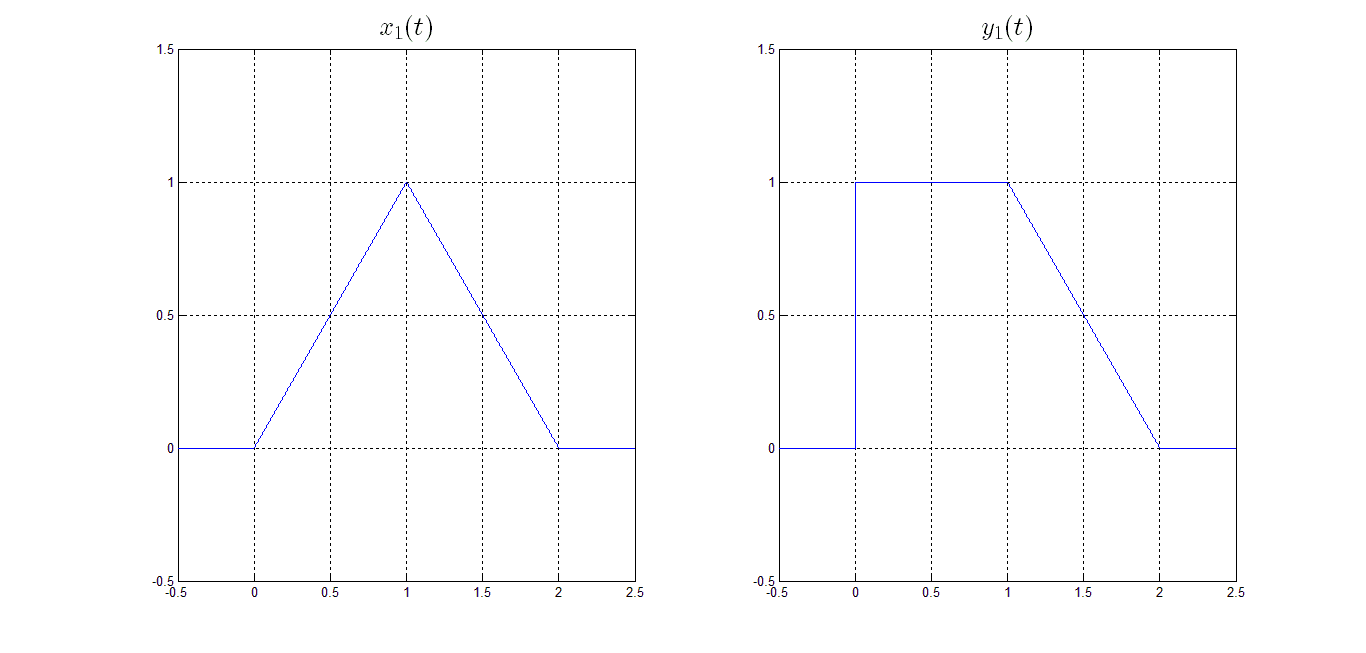
\includegraphics[width=1\textwidth]{./lab3prob2a.png}
            \end{center}
        \end{figure}

        Hallar las respuestas del sistema anterior a las siguientes excitaciones:

        \begin{figure}[H]
            \begin{center}
                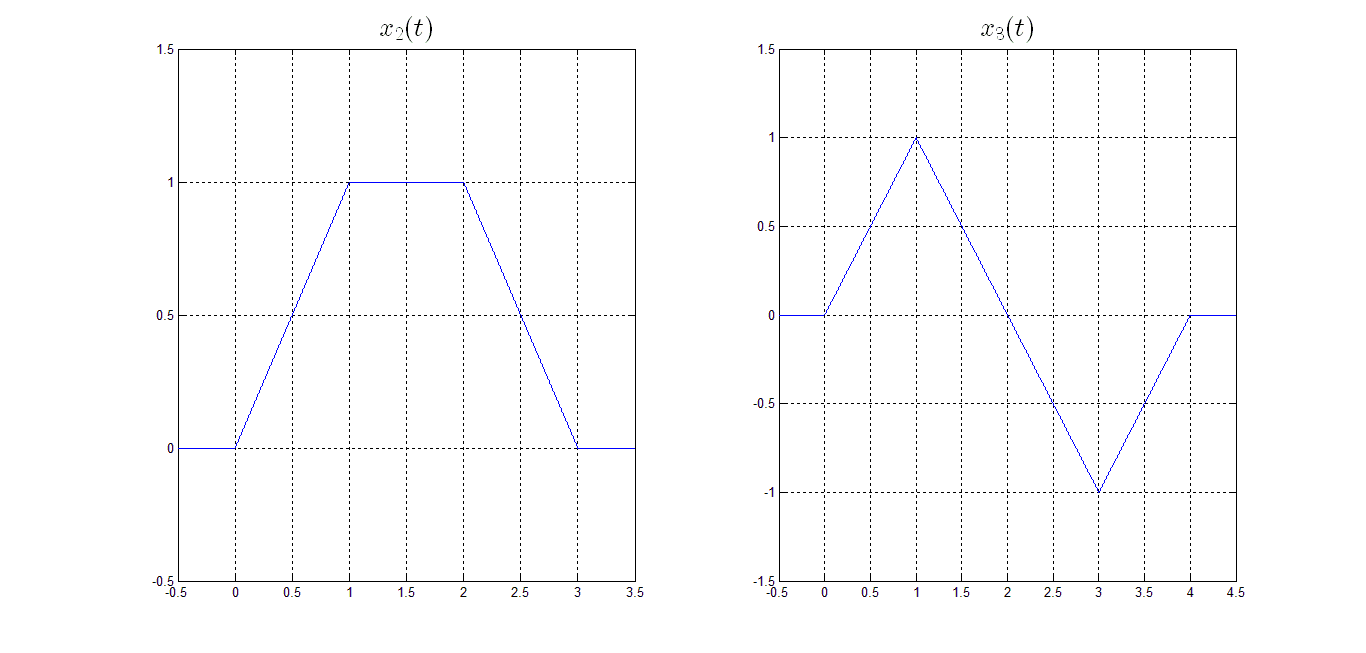
\includegraphics[width=1\textwidth]{./lab3prob2b.png}
            \end{center}
        \end{figure}

        \item Calcular la convolución entre los siguientes pares de señales:
        \begin{enumerate}
            \item $x\left(n\right) = \left(\frac{1}{2}\right)^n u\left(n-4\right)$ y $h\left(n\right) = 4^n u\left(2-n\right)$
            \item $x\left(n\right) = u\left(-n\right) - u\left(-n-2\right)$ y $h\left(n\right) = u\left(n-1\right) - u\left(n-4\right)$
            \item $x\left(n\right) = u\left(n\right)$ y $h\left(n\right) = \left(\frac{1}{2}\right)^{-n} u\left(-n\right)$
            \item $x\left(t\right) = \exp\left(-at\right) u(t)$ y $h(t) = exp(-at) u(t)$
        \end{enumerate}

        \noindent Donde $u\left(n\right)$ es la función escalón unitario.

        \item Para el diagrama de bloques mostrado

        \begin{figure}[H]
            \begin{center}
                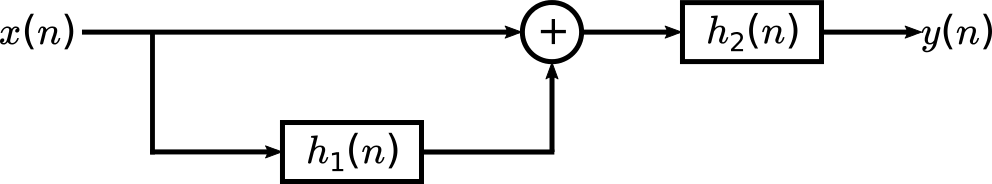
\includegraphics[width=0.8\textwidth]{./lab3prob4.png}
            \end{center}
        \end{figure}

        Donde
        $$h_1\left(n\right) = \beta\delta\left(n-1\right)$$
        y
        $$h_2\left(n\right) = \exp\left(\alpha\right)\delta\left(n\right)$$

        \begin{enumerate}
            \item Escribir la ecuación en diferencias que relaciona la entrada con la salida
            \item Hallar $\alpha$ y $\beta$, de tal forma que la salida sea el promedio entre la entrada en el instante $n$ y
            la entrada en el instante $n-1$.
        \end{enumerate}

        \item Dada la siguiente ecuación en diferencias
        $$y\left(n\right) = -a y\left(n-1\right) + b x\left(n\right) + c x\left(n-1\right),$$
        realizar una representación en diagrama de bloques.

        \item Realizar en \textsc{Matlab} la convolución del siguiente par de
        señales:

        \begin{enumerate}
            \item $x\left(n\right) = \left(-1\right)^n \left(u\left(n\right) - u\left(-n-8\right)\right)$
            \item $h\left(n\right) = u\left(n\right) - u\left(n-8\right)$
        \end{enumerate}

        Graficar la señal resultante, $y\left(n\right) = x\left(n\right) * h\left(n\right)$.
        Usar el comando \texttt{stem}.

        \item Considere un sistema lineal e invariante en el tiempo, causal,
        cuya entrada $x\left(n\right)$ y salida $y\left(n\right)$ estén
        relacionadas por la ecuación de diferencias:
        $$y\left(n\right) = 0.25 y\left(n-1\right) + x\left(n\right)$$
        Determine $y\left(n\right)$ si $x\left(n\right) = \delta\left(n-1\right)$.
        Grafique en \textsc{Matlab} la salida $y\left(n\right)$, use el comando \texttt{stem}.
    \end{enumerate}

\end{document}

